\documentclass[12pt,oneside,openany,letterpaper]{article}


\usepackage{fancyhdr}
\usepackage{helvet}
\usepackage{amsmath}
%\usepackage{graphicx}
\usepackage{psfrag}
\usepackage{setspace}
%\usepackage[hypertex, linktocpage]{hyperref}[2003/11/30]
\usepackage[linktocpage]{hyperref}[2003/11/30]
\usepackage{lscape}
\usepackage{nicefrac}
\usepackage{mathrsfs}
\usepackage{units}
\usepackage{upgreek}
\usepackage{amssymb}
\usepackage{color}
\usepackage{wrapfig}
\usepackage{multirow}
\usepackage{url}
\usepackage{verbatim}
\usepackage[pdftex]{graphicx}
\usepackage{epstopdf}
\usepackage{enumitem}


\onehalfspacing \setlength\textheight{667pt}
\setlength\textwidth{506pt} \setlength\oddsidemargin{-18pt}
\setlength\topmargin{-20pt}
%\setlength\footskip{24pt}
\addtolength\headheight{2.5pt} \addtolength\headsep{-14pt}
%\fancyhead[R]{\includegraphics[height=10.5pt]{ubclogo_bw.eps}\#:  55907968}
%\renewcommand\familydefault{\sfdefault}


%\fancyhead[L]{Name:} \fancyhead[R]{Student
%Number:~~~~~~~~~~~~~~~~~~~~~~~~~~~~~~~~~~~~~~~~~~}
\fancyhead[L]{\emph{Introduction to Electronics}}\fancyhead[R]{Digital Basics}
\fancyfoot[L]{PHYS 231}\fancyfoot[R]{Experiment 7}
\pagestyle{fancy} \pagenumbering{arabic}


\newenvironment{packed_enum}{
\begin{enumerate}
  \setlength{\itemsep}{0pt}
  \setlength{\parskip}{0pt}
  \setlength{\parsep}{0pt}
}{\end{enumerate}}


\newenvironment{packed_item}{
\begin{itemize}
  \setlength{\itemsep}{0pt}
  \setlength{\parskip}{0pt}
  \setlength{\parsep}{0pt}
}{\end{itemize}}


\begin{document}

\thispagestyle{plain}
\begin{center}
{\large{\bf{\fontfamily{phv}\selectfont Physics 231 - Digital Basics (Exp.~7)}}}
\end{center}

\noindent Digital electronics is based on the binary number system. Instead of having signals which
can vary continuously as in analog circuits, digital signals are characterized by only two
voltage levels, typically either 0 volts or +5 volts. The 0 volt level (LO) represents the
binary ``0" or logic ``false" and the +5 volt level (HI) represents the binary ``1" or logic
``true". The simplest digital circuit is the inverter. This device converts a binary $0\to  1$
and a binary $1\to 0$. The function of this device is best illustrated in the following
``truth table". The inversion of a signal $A$ is often represented by $\overline{A}$. Thus in the truth
table for the inverter, $OUT = \overline{IN}$.

\begin{center}
\begin{minipage}[c]{0.3\textwidth}

\includegraphics[width=4 cm]{inverter.eps}
\end{minipage}
\begin{minipage}[c]{0.25\textwidth}
\begin{tabular}{c|c}
$A$ & $Q=\overline{A}$\\
\hline
 0 & 1\\
  1 & 0
\end{tabular}
\end{minipage}
\end{center}

\noindent The function of all digital circuits can be completely described by appropriate truth tables.  The inverter and the other logic gates described below are provided as Integrated
Circuits (IC), packages which usually contain more than one such device. The IC's which
you will use in this experiment are called silicon-gate CMOS FET’s (Complementary
Metal Oxide Semiconductor Field Effect Transistor), and are members of the ``MC54/74"
series. For example, the MC54/{\bf 74HC14}A data sheet provided on the course website
shows that this particular IC contains six inverters. The pin connections for each are also
shown. In addition to the signal connections, {\bf all of the IC's must be connected to both
ground and a +5~V power supply}.

~

\noindent Another digital circuit frequently encountered is the AND gate. This device typically has
two inputs (but can have more) and one output whose value is the logical ``AND" of its two
inputs. For this reason, such circuits are also called “logic gates”. The AND function is
described in terms of the following ``truth table". In terms of logic symbols, $Q = A \bullet B$, where $Q$ labels the output of the logic gate.

\begin{center}
\begin{minipage}[c]{0.3\textwidth}

\includegraphics[width=4 cm]{and.eps}
\end{minipage}
\begin{minipage}[c]{0.25\textwidth}
\begin{tabular}{cc|c}
$A$ & $B$ & $Q=A\bullet B$\\
\hline
 0 & 0 & 0\\
 0 & 1 & 0\\
 1 & 0 & 0\\
 1 & 1 & 1
\end{tabular}
\end{minipage}
\end{center}


\clearpage 

\noindent Still another basic logic device is the OR gate whose output is the logical OR of its
inputs. Thus, $Q = A+B$.

\begin{center}
\begin{minipage}[c]{0.3\textwidth}

\includegraphics[width=4 cm]{or.eps}
\end{minipage}
\begin{minipage}[c]{0.25\textwidth}
\begin{tabular}{cc|c}
$A$ & $B$ & $Q=A+B$\\
\hline
 0 & 0 & 0\\
 0 & 1 & 1\\
 1 & 0 & 1\\
 1 & 1 & 1
\end{tabular}
\end{minipage}
\end{center}

\noindent The industry standard for AND and OR gates, however, are the ``inverting" forms referred
to as NAND and NOR gates respectively. The meaning of the first ``N" is ``Not". Thus,
a NAND gate performs the ``Not AND" function. The small circles at the outputs in the relevant
schematics indicate that the signals at those points are ``inverted", that is a ``1" is
transformed into a ``0", and vice-versa, as demonstrated in the truth tables shown for these
devices. The reason that these are the industry standard is that \emph{all} other digital devices can
be constructed from either the basic NAND or NOR gates.

\begin{center}
\begin{minipage}[c]{0.3\textwidth}

\includegraphics[width=4 cm]{nand.eps}
\end{minipage}
\begin{minipage}[c]{0.25\textwidth}
\begin{tabular}{cc|c}
$A$ & $B$ & $Q=\overline{A\bullet B}$\\
\hline
 0 & 0 & 1\\
 0 & 1 & 1\\
 1 & 0 & 1\\
 1 & 1 & 0
\end{tabular}
\end{minipage}
\end{center}

\begin{center}
\begin{minipage}[c]{0.3\textwidth}

\includegraphics[width=4 cm]{nor.eps}
\end{minipage}
\begin{minipage}[c]{0.25\textwidth}
\begin{tabular}{cc|c}
$A$ & $B$ & $Q=\overline{A+B}$\\
\hline
 0 & 0 & 1\\
 0 & 1 & 0\\
 1 & 0 & 0\\
 1 & 1 & 0
\end{tabular}
\end{minipage}
\end{center}

\noindent In addition to the inverter, you are also supplied with an IC containing {\bf four} 2-input
NAND gates, the MC54/{\bf 74HC00}A.

\clearpage

\noindent {\bf CAUTION}: The CMOS FET’s you will be using are very {\bf sensitive to static discharges}.
Care must be exercised to prevent the FET’s from being exposed to charge build-up,
for example by rubbing against clothing. Even electrostatic charge on the body can cause
damage, so to be safe, you should, after you have walked over to your bench, first touch
some grounded metal (the chassis of the ’scope, for example) before touching the IC’s.
Additional useful precautions:
\begin{packed_item}
\item{Beware of plastic. Do {\bf not} place any CMOS device on plastic surfaces. Also avoid
nylon.}
\item{All low impedance equipment (pulse generators, etc.) should be connected to CMOS
inputs only {\bf after} the CMOS device has been powered up. Similarly, this type of
equipment should be disconnected before power is turned off the CMOS devices.}
\end{packed_item}

~

\begin{center}
{\Large{\bf EXPERIMENTING WITH LOGIC GATES}}
\end{center}

\noindent Build your logic circuits using the breadboard, IC’s, and jumper wires. First connect the +5~V ($V_\mathrm{CC}$) and
ground (GND) connections to the IC. Then connect the output signals to the banana
terminals of the breadboard for subsequent feeding to the oscilloscope or DMM’s. The
IC input signals can be connected to the fixed supply voltages for HI and LO inputs.
\begin{enumerate}[label={\bf\Alph*})]
\item{Verify the truth table for one of the gates available in the laboratory.}
\item{Design and assemble an OR gate using only NAND gates. (Note that a NAND gate
can provide ``inverter" operation by connecting both inputs together.) To facilitate the
design, use de Morgan’s theorem: $\overline{A + B} = \overline{A} \bullet \overline{B}$.
Draw a diagram for the circuit and verify your results by measuring the truth tables
for the circuit you constructed.}
\end{enumerate}

\clearpage
{\large{\bf Flip-Flop or Latch}}

~

\noindent The elements you have studied so far, gates and inverters, may be used to carry out logic
operations, but they exhibit no memory capability; that is, their output states depend only
on the instantaneous values of their inputs. Computers require such elements to carry out
the processing functions (ordinary arithmetic and Boolean algebraic functions) required in
the central processor.

~

\noindent In addition to these devices, however, a computer also requires elements which exhibit
``memory" and act like two-state toggle switches, having outputs that can be set to a
particular state by some transient input and remain in that state after the transient
disappears. One such element of this kind is the {\bf flip-flop}; it has an output, either HI or
LO (1 or 0) which can be switched from one state to the other by applying an appropriate
transient input. Flip-flops are used to perform various memory and arithmetic operations
in computers.

~

\noindent Construct the following circuit from a pair of gates in the {\bf 74HC00} Quad 2-input NAND
gate IC and a pair of inverters.
\begin{center}
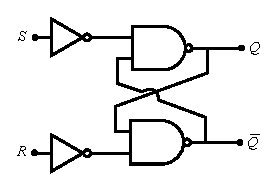
\includegraphics[width=8 cm]{flipflop.eps}
\end{center}

\noindent Supply the $S$ (``Set'') and $R$ (``Reset'') inputs with either HI and LO signals. Connect the
$Q$ and $\overline{Q}$ outputs to the two (dc coupled) vertical inputs of a oscilloscope or DMM. Note
that the state of the outputs is well-defined if either (or both) of the $S$ and $R$ inputs is HI
(5~V). Note also that the system can be in {\bf either one} of two stable output states when the
two inputs ($R$ and $S$) are {\bf both LO} (0~V). In which of these two states it finds itself
depends on which of $S$ or $R$ was {\bf last} set to HI before being returned to LO. Verify these
characteristics of the $RS$ flip-flop.

\clearpage

{\large{\bf Counters}}

~

\noindent A single flip-flop can be used as a memory element and can also be used as the starting
point for a counter, although it can only count from zero to one, since it can only store
one “bit” of information. In this final section, you will investigate the use of a decade
counter, an IC capable of counting to from 0 to 9.

~

\noindent We will use the MC74HC390 ``Dual 4-Stage Binary Ripple Counter with $\div 2$ and $\div 5$
Sections'' for a pair of decades. This IC contains {\bf two} decade counters, each consisting
of four flip-flops, one a $\div 2$ counter, and the other three constituting a $\div 5$ counter. When these two counters are connected together they form a counter capable of counting from
zero to 9, a ``Binary Coded Decimal'' counter.  The single IC contains two such decimal counters, one on each side of the chip.

~

\noindent The flip-flops internal to this counter are triggered by HI-to-LO transitions of the
``clock" pulses. Commercial counter chips such as these also possess a ``Reset" input to
enable resetting the counter to ``zero" when a suitable pulse is applied. In the 74HC390, the required reset pulse is of positive polarity (from LO to HI and back).  
\begin{comment}
The ``reset-to-zero" inputs of the 74LS90 are labelled ``R0(1)" and ``R0(2)".  The 74LS90 also has inputs that can be used to set the outputs  of the counters to 1.  These inputs are labelled ``R9(1)" and ``R9(2)". In normal operation, all of R0(1), R0(2), R9(1), and R9(2) should be held LO (i.e.\ grounded).
\end{comment}
In normal operation the reset inputs should be held LO (i.e.\ grounded).
Verify the counting characteristics of the 74HC390 IC by examining the sequential ``truth table" (counting sequence) using a series of pulses (obtained from the function
generator TTL output) as a clock input.

~

\noindent Monitor the state of the counter (the outputs labelled “Q” on the pin diagram) using
indicator lights (LED’s). Place a resistance of approximately $200~\Omega$ between the LEDs
and the counter outputs to limit the current. First try the $\div 2$ counter, then the $\div 5$ counter.
Try wiring together these two to make a binary coded decimal counter. Don't forget to include wiring diagrams
in your notebook.

\end{document}
